\section{Introduction}
JavaScript is one of the most widely used programming languages not only for
client-side but also for server-side programming~\cite{nodejs, meanjs} and even
for small embedded systems~\cite{espruino, tessel2}.  It is the top-ranked
language used in active GitHub repositories\footnote{https://githut.info/}, and
\#7 in the TIOBE Programming Community
index\footnote{https://www.tiobe.com/tiobe-index/}.  According to
W3Techs\footnote{https://w3techs.com/technologies/details/cp-javascript/all/all},
95.0\% of websites use JavaScript as their client-side programming language.

Despite its popularity, JavaScript developers often suffer from its intricate
semantics, which may cause unexpected behaviors.  For example, calling the
following JavaScript function seems to always return \( \code{false} \):
\begin{lstlisting}[style=myJSstyle]
function f(x) { return x == !x; }
\end{lstlisting}
Unfortunately, it returns \( \code{true} \) when its argument
is an empty array \( \code{[]} \).  To correctly understand and reason about
such a complex behavior, the formal semantics of JavaScript is necessary.

\begin{figure}
  \centering
  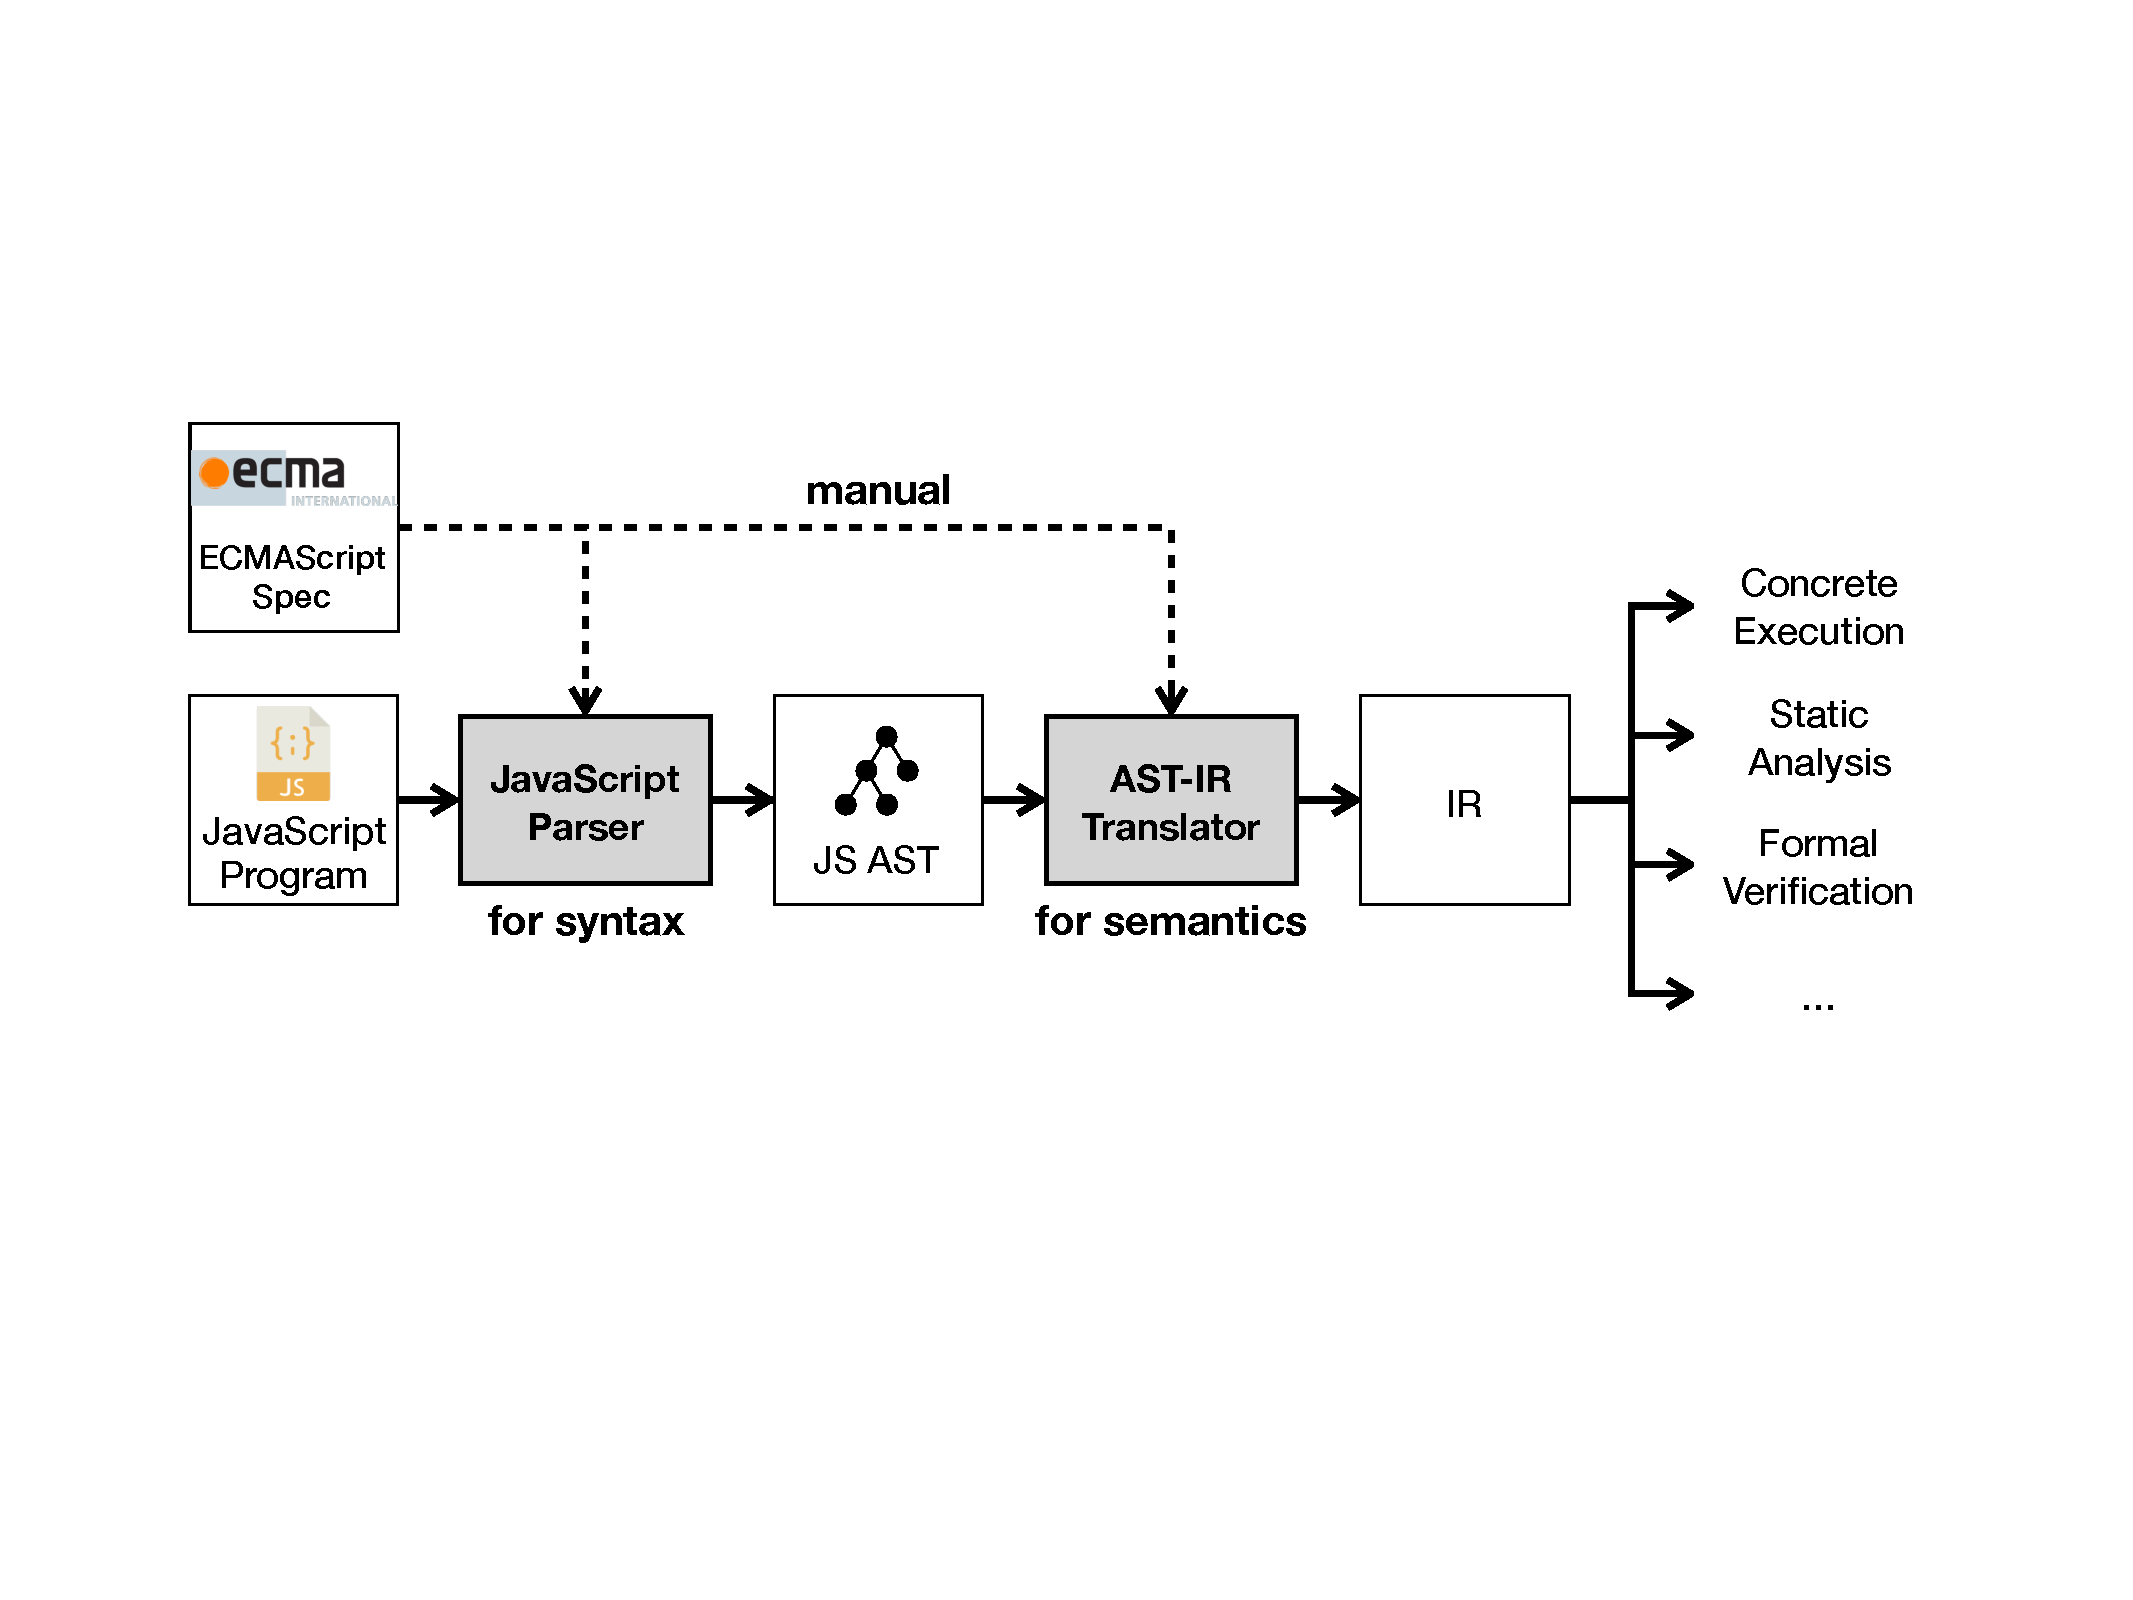
\includegraphics[width=0.48\textwidth]{img/existing.pdf}
\vspace*{-2em}
  \caption{Existing approaches: Manually built parsers and AST-IR
  translators for JavaScript IR-based semantics}
  \label{fig:existing}
\vspace*{-1em}
\end{figure}

Researchers have defined various JavaScript formal
semantics~\cite{aplas08,lambdajs,kjs,javert} suitable for static
analysis~\cite{jsai,tajs,wala,safe} and formal verification~\cite{javert} by
referring to ECMAScript.  ECMAScript is the official specification that
describes JavaScript syntax using a variant of the extended BNF (EBNF) notation,
and its semantics using abstract algorithms written in English in a clear and
structured manner.  \textit{IR-based semantics extraction} is a typical way to
define the formal semantics by building a compiler from programs to Intermediate
Representations (IRs) to indirectly represent the semantics of given programs.
As illustrated in Figure~\ref{fig:existing}, the compiler consists of a parser
that constructs Abstract Syntax Trees (ASTs) of given JavaScript programs, and
an AST-IR translator that converts ASTs to their own IRs.  This approach helps
researchers focus on IRs without worrying about diverse and enormous features of
JavaScript in developing new techniques for static analysis and formal
verification.

However, to the best of our knowledge, all existing approaches to JavaScript
IR-based semantics extraction \textit{manually} build parsers and translators.
Although it was reasonable approach until ECMAScript 5.1 (ES5.1,
2011)~\cite{es5}, the manual approach is too tedious, labor-intensive, and
error-prone to deal with the large size of modern JavaScript since ECMAScript 6
(ES6, 2015)~\cite{es6}. ES6 introduced lots of significantly new features such
as lexical binding via \( \code{let} \), the spread \( \code{...} \) operator,
classes, the \( \code{for-of} \) operator, the \( \code{async} \) functions, and
generators.  KJS~\cite{kjs} is one of formal semantics of ECMAScript 5.1 (ES5.1,
2011) and it is defined on top of \( \kframework \), which is a framework for
defining language semantics.  According to an author of KJS, it took
\textit{four months} to implement AST-IR translator for 1,370 steps out of 2,932
steps in 368 abstract algorithms. However, the most recent version of ECMAScript
(ES10, 2019)~\cite{es10} has 1,731 abstract algorithms consisting of 10,068
steps. Thus, it is not scalable to build AST-IR translator for modern JavaScript
and no formal semantics exists for ES6 to ES10.

Moreover, JavaScript syntax and semantics are annually updated.  Until
ECMAScript 5.1, JavaScript was a stable language because the specification was
rarely updated.  However, The Ecma Technical Committee 39 (TC39)~\cite{tc39}
decided to release the specification annually in late 2014.  After this official
announcement, several syntax features and roughly 1,000 to 3,000 steps of
abstract algorithms are modified or newly added in the specification every year.
To deal with these frequent and massive updates of ECMAScript, researchers
should manually update parsers and AST-IR translators by putting a lot of
effort.

To alleviate this problem, we propose a technique to \textit{automatically
synthesize} parsers and AST-IR translators directly from ECMAScript with
\textit{forward compatibility}. There are several technical challenges in
synthesizing parsers and translators. For syntax, ECMAScript utilize their own
special variant of the EBNF with parametric non-terminals, conditional
alternatives, and various special terminal symbols.  Thus, no existing parser
generation technique is directly applicable for this variant.  Moreover,
JavaScript provides automatic semicolon insertion in its parsing algorithm with
several complex rules not in a lexer. For semantics, abstract algorithms in
ECMAScript are written in English.  Besides, general and forward compatible
representation of abstract algorithms is necessary for future version of
ECMAScript.

Our contribution is \( \tool \), a JavaScript IR-based Semantics Extraction
Toolchain:
\begin{itemize}[leftmargin=0.5cm]
  \item \( \tool \) is the \textit{first} tool that can automatically synthesize
    parsers and AST-IR translators for modern JavaScript directly from
    ECMAScript.  For syntax, we formalize the variant of EBNF as \( \bnfes \)
    for the first time, and propose a parser generation technique with
    \textit{lookahead parsing} for \( \bnfes \) with automatic semicolon
    insertion. For Semantics, synthesis of AST-IR translators are semi-automatic
    assisted by \textit{compile rules} because of the difficulty in dealing with
    the semantics written in a natural language.  Compile rules describe how
    each step of abstract algorithms is converted into our intermediate
    representation \( \ires \) designed for ECMAScript. We evaluated \( \tool \)
    for the five most recent ECMAScript versions including the draft of the next
    version (ES6 to ES11).  We succeed to generate parsers for all versions, and
    to automatically cover \inred{XX.X}\% of steps in abstract algorithms in
    average.
  \item Based on \( \tool \), we define the first IR-based formal semantics of
    modern JavaScript.  The semantics targets the core part of the draft of next
    version of ECMAScript (ES11), and our tool successfully synthesizes its
    parser and AST-IR translator for \inred{X,XXX} out of \inred{X,XXX}
    algorithm steps.  We manually complete the missing parts of the AST-IR
    translator (\inred{XXX} steps) in \inred{XX} days.  To check the correctness
    of the formal semantics, we evaluated Test262~\cite{test262}, the official
    conformance test suite, and the semantics passed all \inred{XX,XXX}
    applicable tests.  Moreover, we found \inred{X} specification errors in ES11
    based on the formal semantics.  They were all confirmed by TC39 and will be
    fixed in the next release.
  \item \( \tool \) is also forward compatible with new language features
    proposed for future ECMAScript specifications.  TC39 manages proposals of
    new language features in an open source
    project\footnote{https://github.com/tc39/proposals}.  There are five stages
    of proposals (from Stage 0 to Stage 4).  All proposals in Stage 4 (Finished)
    are applied in the draft of the next ECMAScript, Stage 3 (Candidate) is the
    last stage before Stage 3.  For evaluation of forward compatibility of \(
    \tool \), we applied our tool to all \inred{XX} Stage 3 proposals. It
    succeeded to synthesize parsers for all proposals, and to convert \inred{XX}
    out of \inred{XX} algorithm steps for all proposals. After completing all
    missing parts, each semantics passed all \inred{XX} tests.
\end{itemize}
